\documentclass[]{article}
\usepackage{graphicx}

\begin{document}

\title{Analyzing the Number of Updates Sent}
\maketitle
\newpage
The topology used is shown below. \\
\linebreak

\begin{center}
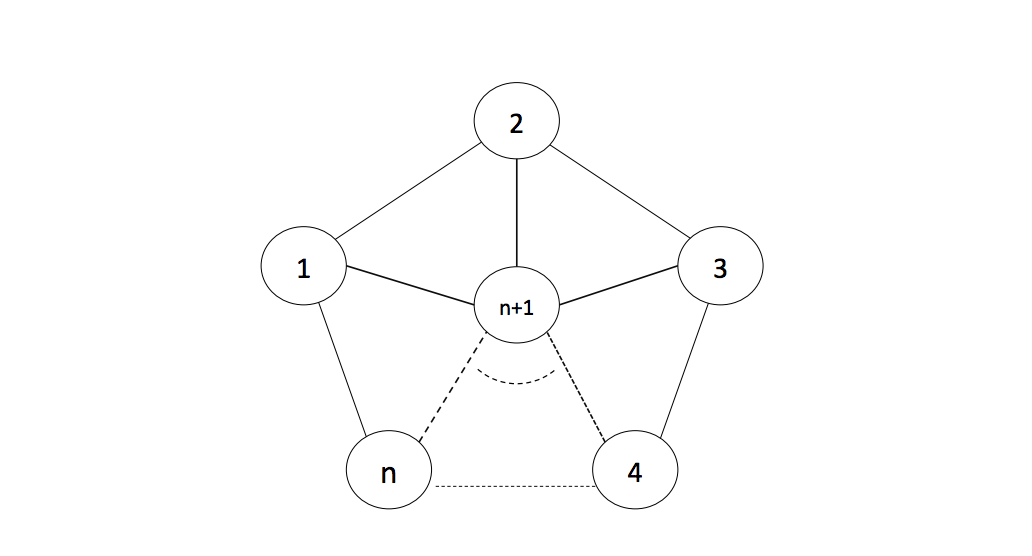
\includegraphics[width=10cm]{topo.png}
\linebreak
The total number of updates sent as a function of the number of routers in the topology is contained in the array: 

[24
38
55
78
102
129
159
192
228
267
309
354
402
453
507
564
624
687
753
822
894
969
1047
1128
1212
1299
1389
1482
1578
1677
1779
1884
1992
2103
2217
2334
2454
2577
2703
2832
2964
3099
3237
3378
3522
3669
3819
3972]
\linebreak

The plot of this data is shown below.
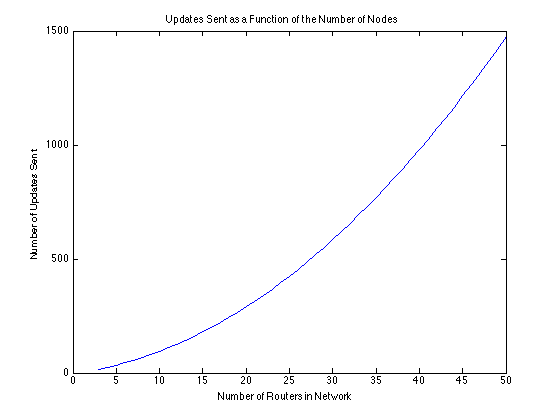
\includegraphics[width=13cm]{plot.png}
\linebreak
As we can see, with my RIPRouter implementation, the number of updates sent is relatively few and grows linearly as the number of routers in the network grows. This is fantastic, as we have a convergence time that scales proportionally with the number of routers in the network.
\end{center}
\end{document}